\chapter{Background}
This chapter provides background information on Wireless Networks and recalls some graph-theoretic basics we used in our work.
At first we will take a look at the relevant points of APs followed by illustrating the bigger picture on how to use those
within a network. Then, we examine the way APs communicate with each other through channels, how those communications are affected by interference, and
how to access the shared medium. Finally, we will outline the implementation of the \ac{WDS} we are optimizing.
In the second part, we explain spanning trees on graphs and depict graph attributes like edge- and vertex-connectivity.
Subsequently, we will give a detailed description of how we map a real world \ac{AP}-infrastructure-setup to network graphs in order 
to compute a solution and conclude this part by discussing the relevance of the problem COLORING for our approach.

\section{Wireless Networks}
  Wireless networks are computer networks which use radio-waves for communication.
  They are used in scenarios where using wires is not possible or cumbersome like systems where devices are mobile or subject to drastic link-quality changes.
  There are different scales where wireless networks are utilized:
  \begin{itemize}
    \item Smaller systems like a \ac{PAN} where a smartphone uses Bluetooth to connect to headphones. The typical range lies within a couple of meters.
    \item Medium sized systems like a \ac{WLAN} with laptops or smartphones connecting to an infrastructure through a wireless \ac{AP}.
      The typical range is up to 100 meters.
    \item Large scale systems like television broadcasting with \ac{DVB-T} through satellites with ranges of up to 35,400 kilometers.
  \end{itemize}
  
  We will focus on medium sized systems in our work.

  \subsection{Accesspoints}
    A wireless \ac{AP} is a device which allows \ac{WLAN}-clients to connect to its network.
    Typically it serves as an entry point to a network-infrastructure and ultimately the internet like a common network switch, 
    but APs can also be used in different ways. In the following we will describe the modes we use APs in:
    
    \begin{description}
      \item[Infrastructure-mode:]
	Using this mode, the clients connect themselves to the APs in order to get access to the network behind the APs, like fileservers or the internet.
	To do so one or more APs announce their services through small broadcasted packets called beacons, which include a \ac{SSID}, 
	the name/identifier of the wireless network. Those are used to differentiate multiple wireless networks from each other if used in the same area. 
	SSIDs, if received, are then used by the clients to establish a link to the APs.

      \item [Point-to-Point mode:]
	This mode is defined by a static link between exactly two interfaces in contrast to infrastructure- and ad-hoc- mode, where this affiliation is not determined.
	It allows an \ac{AP} to create a dedicated link to another \ac{AP} using the same mode. This link would consequently be shared only by these two APs,
	additionally the transmitted data is encrypted. This mode is useful in scenarios where complex connection-constellations can not be achieved by 
	client-infrastructure-mode combinations solely. Alternatively, one could also use the ad-hoc mode, which was not available, as it was not implemented yet in LANCOM devices.
	
      \item [Client-mode:]
	Here the \ac{AP} behave the same as ordinary clients like laptops or smartphones.
	They search for wireless networks announced by APs in infrastructure mode and connect themselves to these.
	Often this mode is used to enable devices which lack 802.11-hardware to access a \ac{WLAN} through a wired link to those APs.
    \end{description}
    
    \begin{figure}[bh!]
      \centerline{
	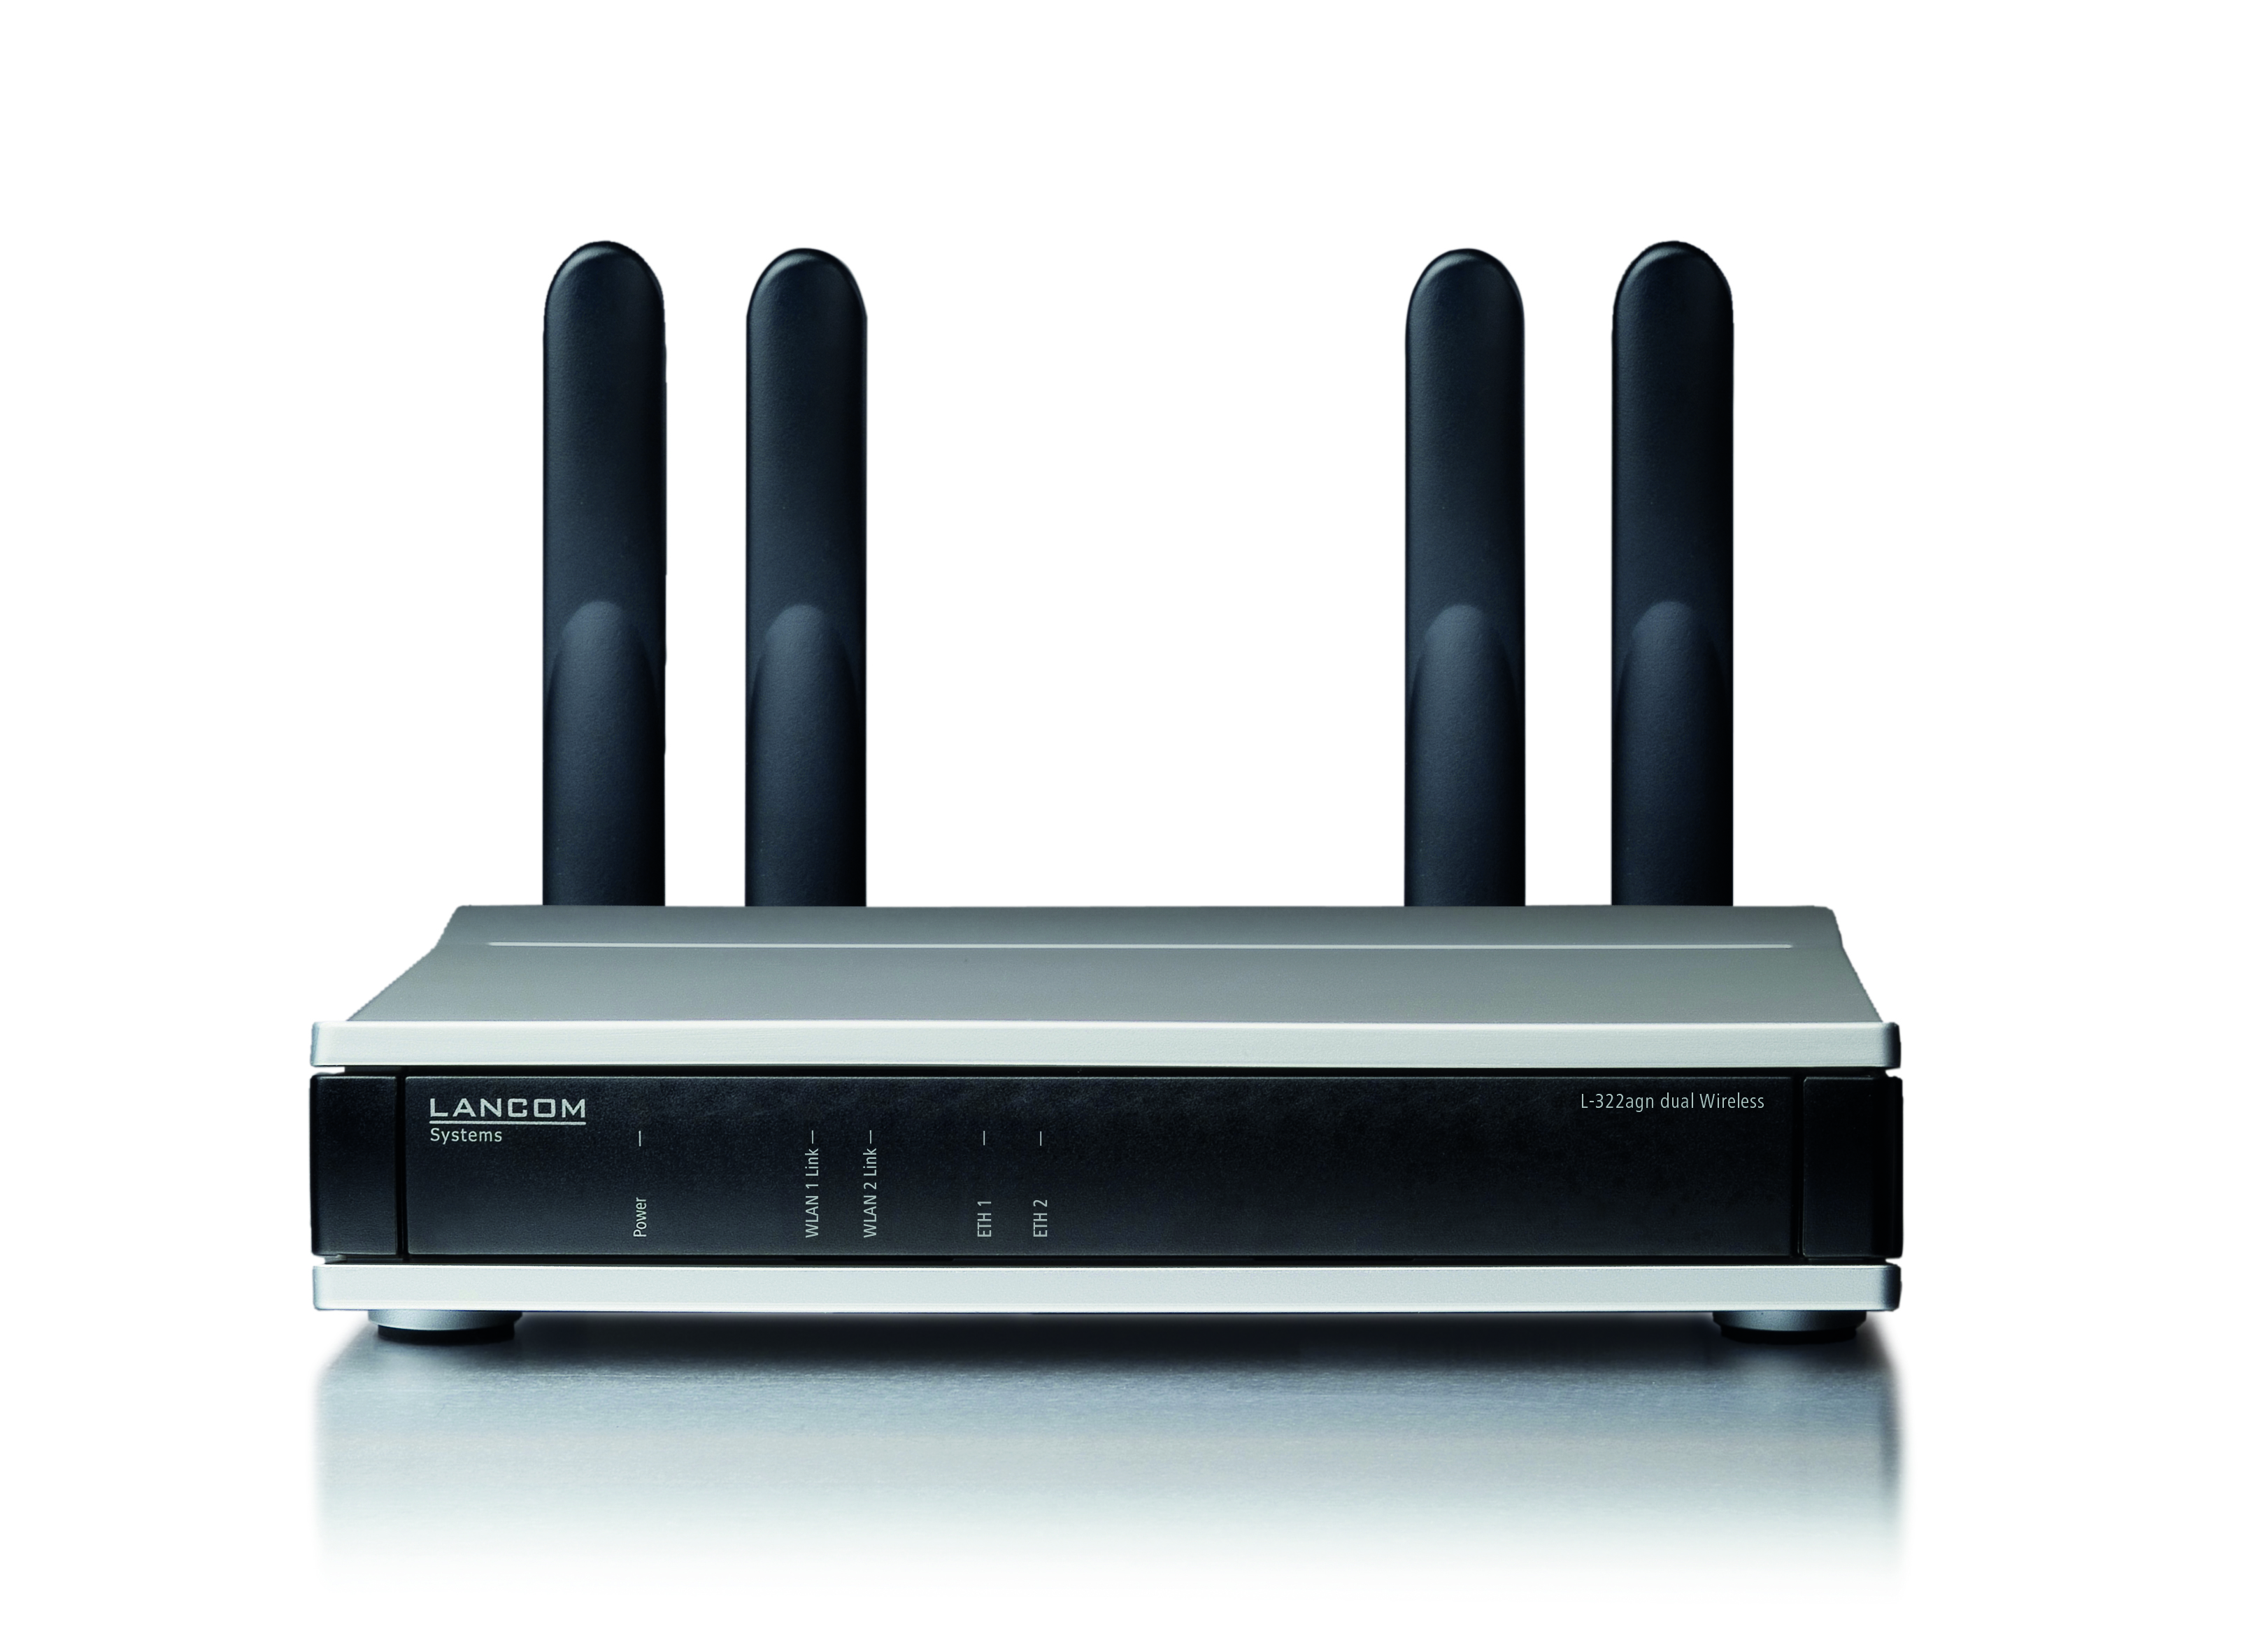
\includegraphics[width=0.5\textwidth]{figures/L-322agn.jpg}
	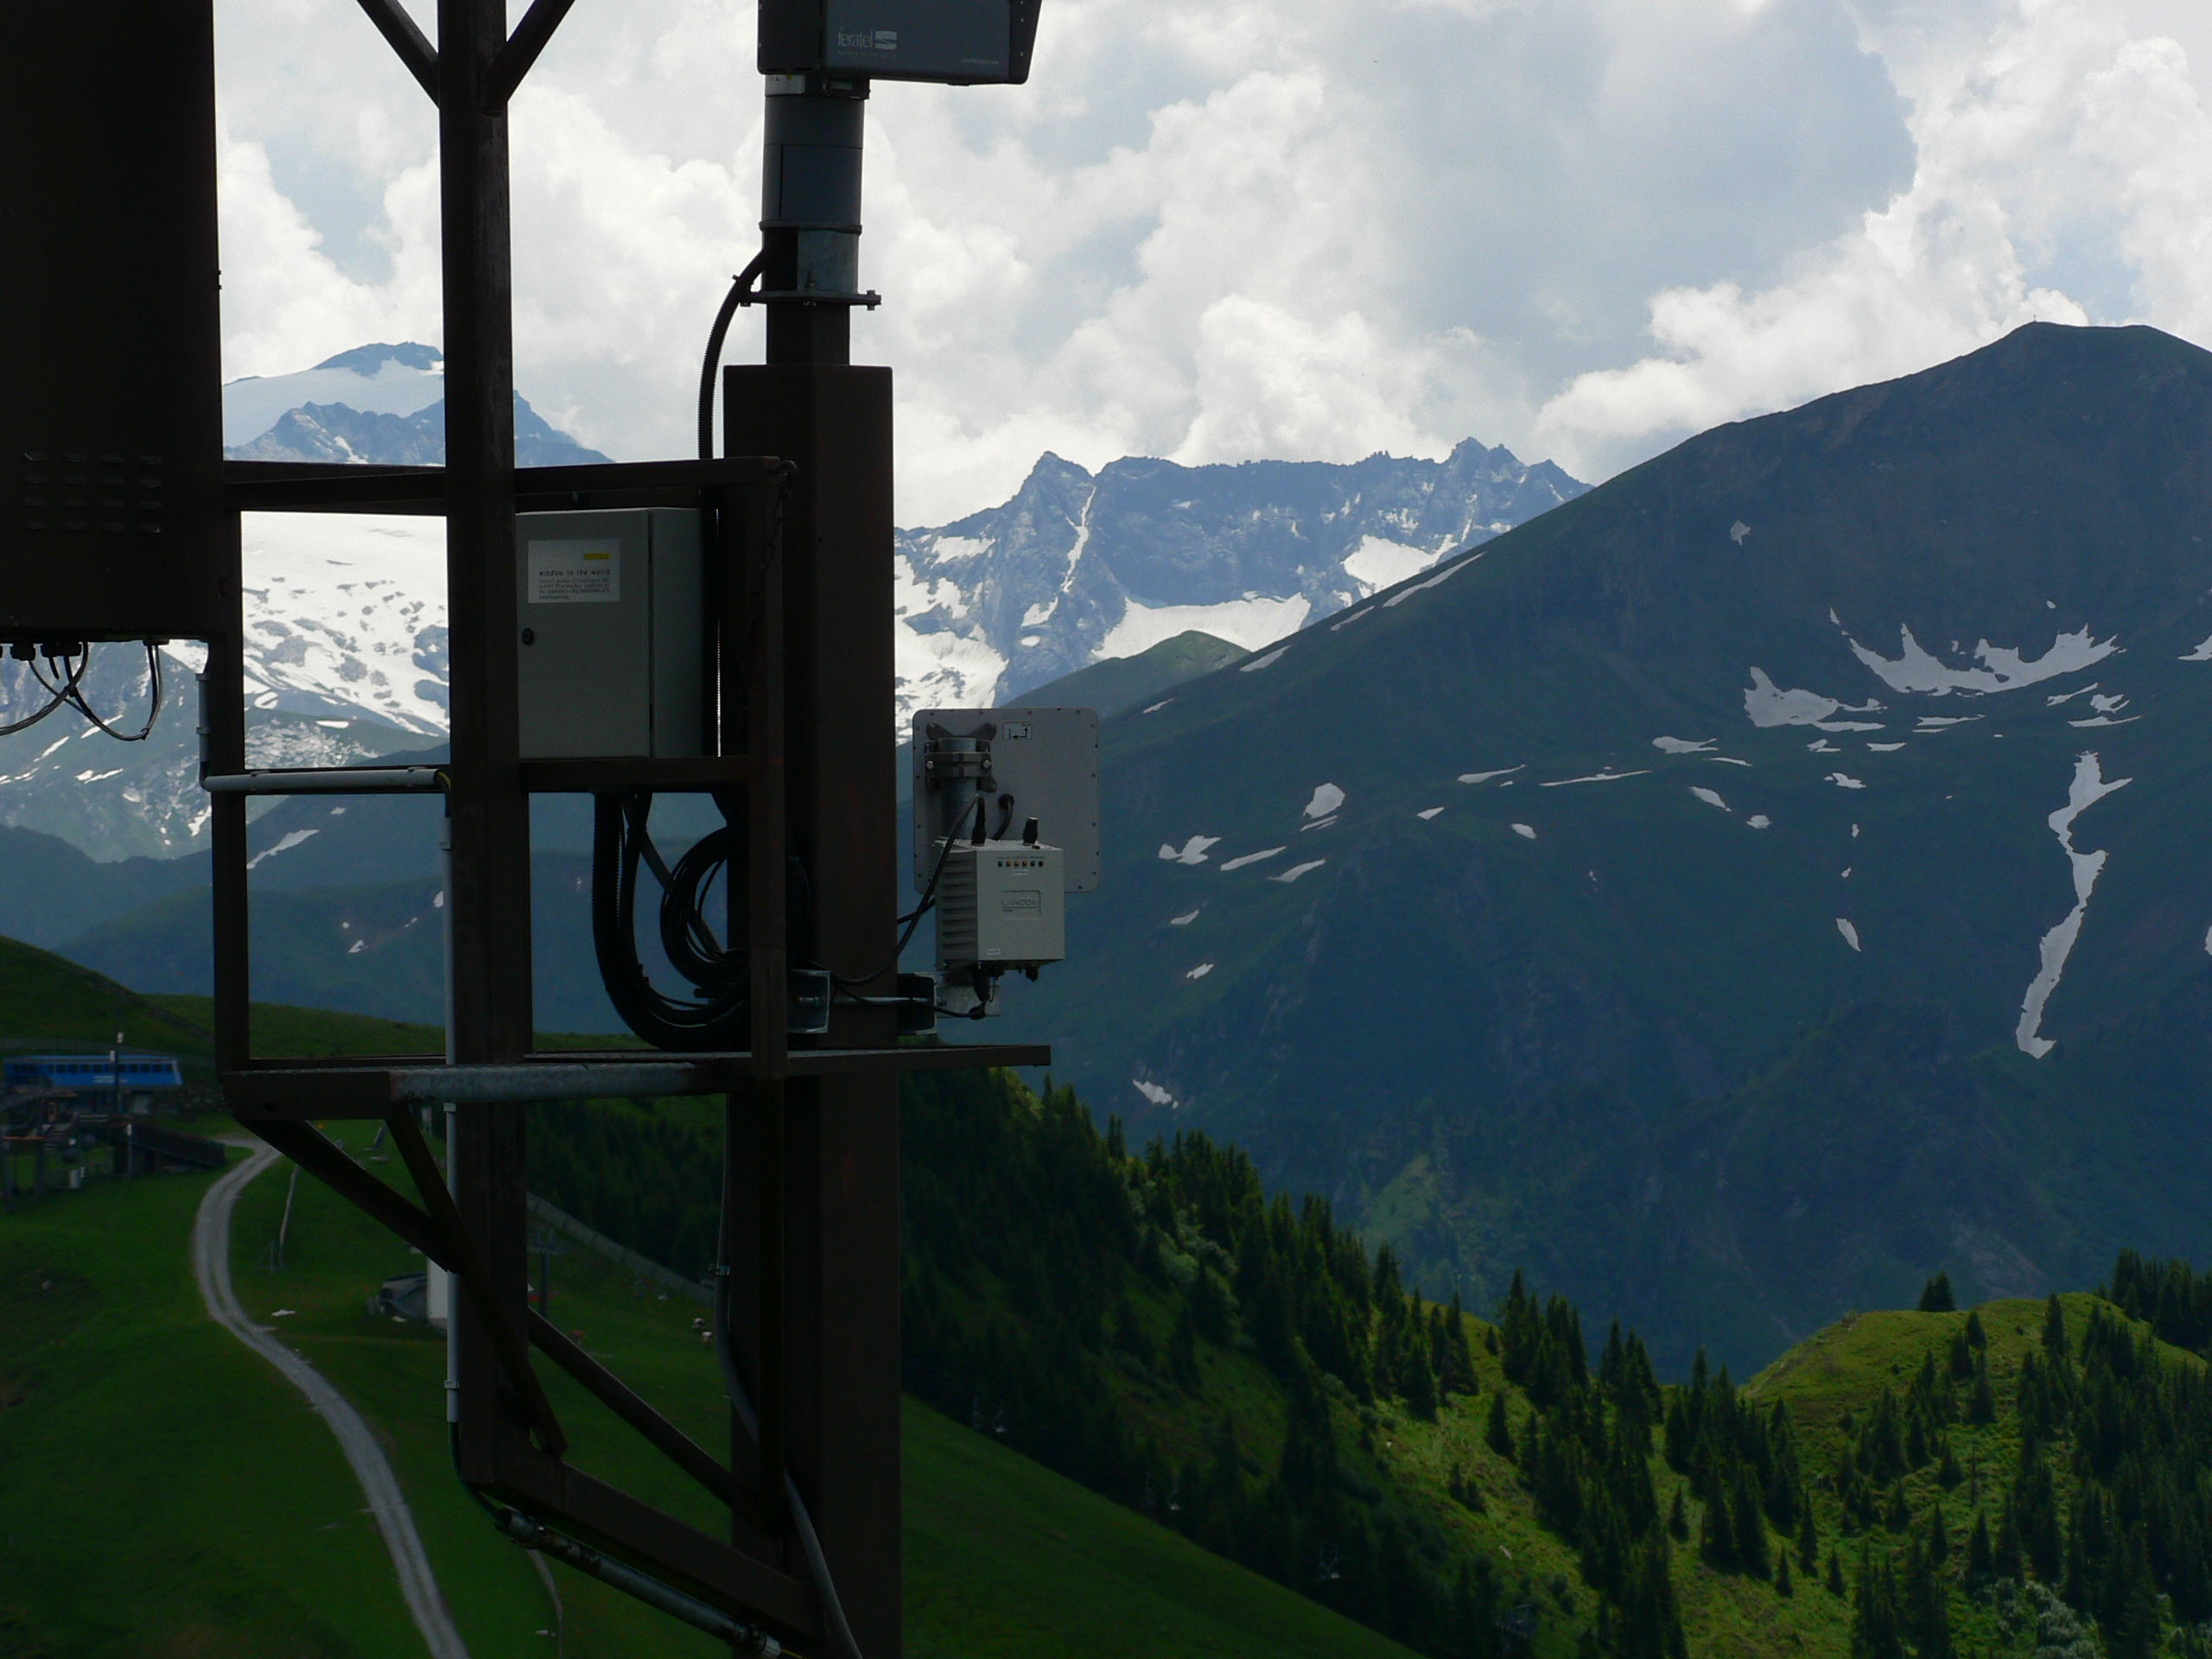
\includegraphics[width=0.5\textwidth]{figures/outdoor_berge.JPG}
      }
      \caption{Indoor \ac{AP} (left) and an outdoor version deployed (right) \cite{lancom}.}
      \label{fig:L-322agn}
    \end{figure}
    
    \newpage
     
  \subsection{Channel}
    A \ac{WLAN} channel as specified by the IEEE 802.11 family uses a specific frequency-range in the \ac{UHF} or \ac{SHF} radio-scope in order 
    to modulate data digitally on carrier waves.
    Doing this allows transmitting data from a sender station to a receiver station and creates a network-link between them.
    \ac{WLAN} uses two license-free frequency bands at 2.4 GHz and additionally bands around 5 GHz.
    As we can see in figure \ref{fig:wlan_channels}, channels have overlapping regions, which can lead to conflicts.
    Two independent pairs of radios in the same area can communicate almost free of interference, if they use different, non-overlapping channels.
    Newer APs may use channels with 40 MHz bandwidth in order to further increase throughput with the drawback of creating more overlapping frequency-regions
    and therefore possibly creating sources of interference for other channels close-by.
    The overlapping regions are a problem especially in the 2.4 GHz band, but if wider versions of channels in the 5 GHz band are used, also those are affected,
    although not as bad as in the 2.4 GHz, where the channels overlap per even at 20 MHz width.
    
    \begin{figure}[bh!]
      \centering
      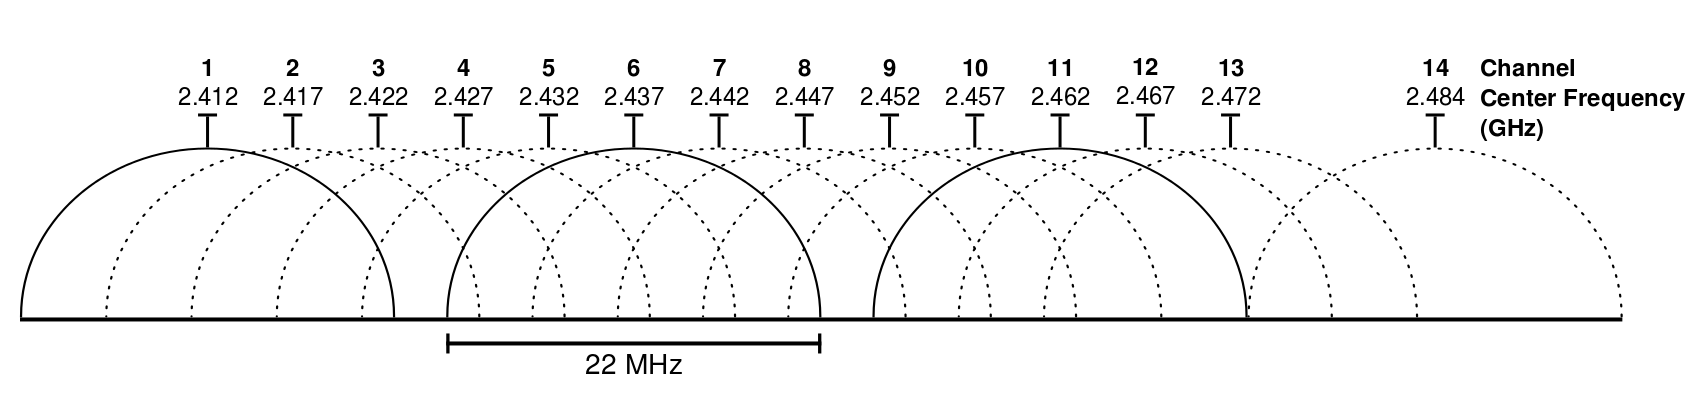
\includegraphics[width=\columnwidth]{figures/wlan_channels.png}
      \caption{Mapping of channels to frequencies for the 2.4GHz band \cite{wlan_channels}.}
      \label{fig:wlan_channels}
    \end{figure}
    
    \begin{figure}[bh!]
      \centering
      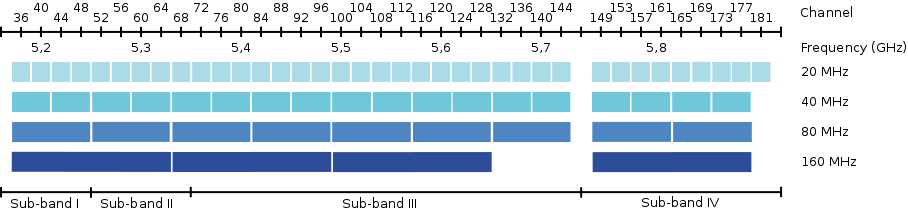
\includegraphics[width=\columnwidth]{figures/5ghzband}
      \caption{Channels in the 5 GHz band with different channel width.}
      \label{fig:5ghzband}
    \end{figure}
    
      \subsubsection{CSMA / CA}
	\ac{CSMA/CA} is a network protocol that describes how to access a shared medium, like a shared \ac{WLAN} channel.
	It behaves as described by \cite{csma_techo}:
	
	\begin{quotation}
	  CSMA works on the principle that only one device can transmit signals on the network, 
	  otherwise a collision will occur resulting in the loss of data packets or frames. 
	  CSMA works when a device needs to initiate or transfer data over the network. 
	  Before transferring, each CSMA must check or listen to the network for any other transmissions that may be in progress. 
	  If it senses a transmission, the device will wait for it to end. Once the transmission is completed, 
	  the waiting device can transmit its data/signals. However, if multiple devices access it simultaneously and a collision occurs, 
	  they both have to wait for a specific time before reinitiating the transmission process. 
	\end{quotation}
	
	For a sizeable \ac{AP}-deployment the accumulated backoff-waiting times increase as more data is transmitted and backoff-timers are triggered more often.
	This effect also quickly degrades network performance, especially in a mono-channel setup.
	
	Another interesting, but undesired effect in accessing the medium despite following the CSMA algorithm is the hidden-station-problem.
	It describes a scenario where an \ac{AP} B is in range of A and C, but A and C do not see each other (see \ref{fig:csmaca}).
	Then, if the situation occurs that the two outer APs simultaneously want to send data to the \ac{AP} in the middle, as they can not notice the 
	other AP sending data, their packets collide at B and therefore effectively transmit less or nothing at all, since B is not able to correctly decode the packets.
	The effect is similar to two people talking to a third person at the same time.
	To alleviate the problem the RTS/CTS extension was introduced, which introduces small \ac{RTS}-requests and \ac{CTS}-announcements. 
	This is basically the station/person that is talked to announcing to whom it is going to listen for the next period of time.
	Note that the RTS/CTS not completely solves this problem, but lessens its impact.
	
	\begin{figure}[th!]
	  \centering
	  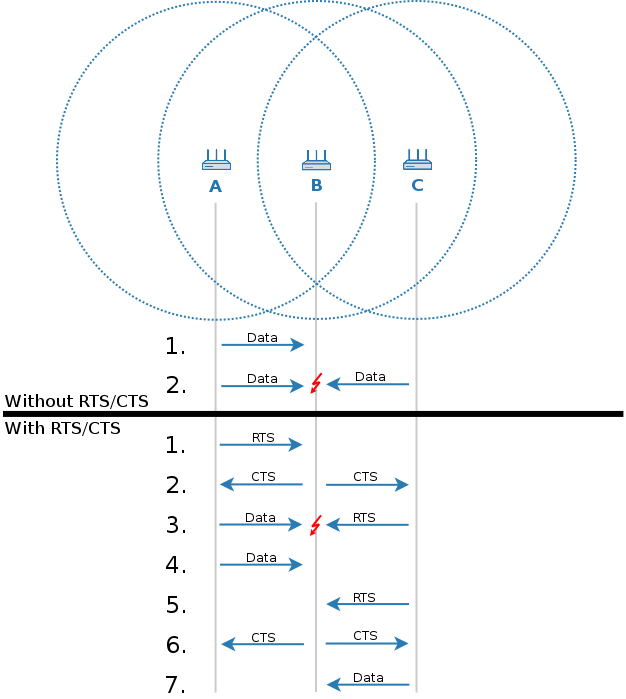
\includegraphics[width=1\columnwidth]{figures/csmaca.png}
	  \caption{Hidden-Station Problem and the RTS/CTS solution. A sends data to B in step 1.
	    Because of the range-limitation, C does not recognize the transmission of A to B. 
	    If B then wants to also transmit data to B, it checks if the medium is free, which it falsely assumes
	    and then starts to transmit its data. This leads to collisions at B in step 2 and the data received will be corrupt.
	    With RTS/CTS: First A asks B if it may send data to it, which B allows by sending the OK to every station listening (A and C). 
	    Then A sends its data to B while C has to wait until B's time slice expires (a CTS defines the amount of time how long a station will listen to another, so there is no
	    need for constant polling). Eventually C succeeds in getting its CTS from A and is able to also transmit its data to B without collisions.}
	  \label{fig:csmaca}
	\end{figure}

      \subsubsection{Interference}
	Wireless interference occurs if two senders at the same time transmit data on the same carrier frequency. If so the waves may interfere and be wrongly detected
	by the receiving stations. This leads to changed bits in the derived data and may result in turn to corrupt messages if more bits are flipped than the
	forward error correction algorithms can detect. Such a malformed packet may not even be recognized as such, if the preamble, which is a certain signal to indicate an
	incoming data stream, is already corrupt, rendering the rest of the packet as unusable noise. If a certain threshold of flipped bits occur after the preamble,
	calculating the checksum on those packets will then show that there have been errors while transmitting the data, which will make the receiving station 
	throw away this packet (destructive interference).
	As the receiving station will not acknowledge the receipt of the packet, the sender will assume the packet was not transmitted correctly and therefore try 
	to send the same packet again. If this process occurs often, throughput performance will suffer as it takes more time to send the same amount of data.
	This kind of interference is called cooperative and occurs if two radios claim the same channel/medium (co-channel/adjacent-channel interference) if CSMA fails,
	like in the hidden-station or exposed-station problem.
	Whereas there is also uncooperative interference from devices like microwaves or cordless phones which do not access the medium purposefully, but rather
	emit noise by accident on the same frequency. Nevertheless, the effect is the same.
	
	For our purposes we generally define interference for wireless connections as any kind of disruption in communication, 
	that includes both cooperative and non-cooperative interference.
	
	Despite solutions like RTS/CTS and others that mitigate the hidden station problem (and alleviate the cooperative interference),
	there are still some situations where collisions and therefore interference occurs.
	Additionally at a certain signal-strength level a station, while doing its carrier sensing, may not be able to differentiate noise from another stations transmission.
	As \cite{padhye2005estimation} mentions, interference is the key cause of performance degradation in wireless networks. Hence, our idea is to increase throughput 
	performance by reducing interference as much as possible.
	
	\begin{figure}[h!]
	  \centering
	  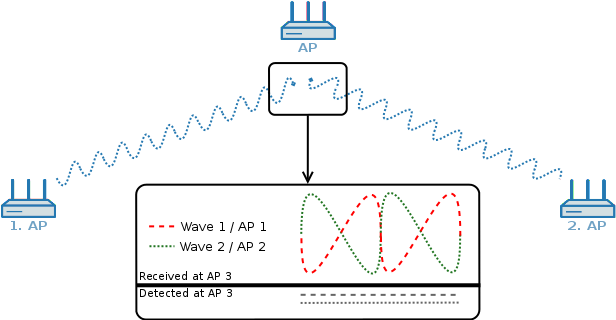
\includegraphics[width=0.8\columnwidth]{figures/interferenz}
	  \caption{Using the same or close-by carrier frequencies, waves may interfere and result in falsely detected bits and render transmitted data corrupt.}
	  \label{fig:interferenz}
	\end{figure}
	
\newpage
	      
    \subsection{Wireless Distribution System (WDS)}
      A \ac{WDS} is defined by \cite{dd_wrt} as a system, that
      
      \begin{quote}
	creates a wireless backbone link between multiple access points that are part of the same wireless network. 
	This allows a wireless network to be expanded using multiple access points without the need for a wired backbone to link them, as is traditionally required. 
	The WDS-enabled \ac{AP} can accept wireless clients (e.g. wireless laptop users) just as traditional APs would.
      \end{quote}

      They also point out, that WDS is currently not a certified standard of the \ac{IEEE} and every vendor implements it in a different way.
      For an example see figure \ref{fig:camping}. The idea behind this system is to make increasing the range of an already pre-configured \ac{WDS}
      easy by just adding another \ac{AP} somewhere in range of the other APs and powering it on.
      Setting up the rest of the infrastructure and configuration from then on is supposed to happen automatically. 
      This system allows us for example to quickly bring a network infrastructure to areas where no 
      existing infrastructures (existing power- or network-cabling) can be utilized for this purpose, without the burden of creating such a costly infrastructure.
      
      \subsubsection{\ac{WLC}}
	The purpose of a \ac{WLC} is to centrally manage and configure multiple APs automatically - effectively ease the job of the administrator responsible for a 
	wireless infrastructure. They are usually located in central networking-cabinets next to other network core components like switches and servers.
	Managing such a \ac{WDS} can also be done through another central entity somewhere else in the network, for example by
	electing an \ac{AP} for this job, which is directly connected to the wired \ac{LAN}, as it is done by DD-WRT \cite{dd_wrt}. 
	Taking it one step further and eliminating the central logic at all would then result in a distributed logic on each of the APs, which is however more complex. 
	We will only deal with the centrally, managed scenario and ignore distributed approaches.
	
	\begin{figure}[h!]
	  \centering
	  
\includegraphics[width=0.7\columnwidth]{figures/wlc}
	  \caption{A LANCOM WLAN Controller \cite{lancom}}
	  \label{fig:wlc}
	\end{figure}
	
	\newpage
      
      \subsubsection{WLC Aided Configuration}
	For a common \ac{WLAN} infrastructure deployment all APs are connected to the wired backbone and use their radios solely in infrastructure mode to 
	offer clients an entry point into the network.
	\begin{figure}[h!]
	  \centering
	  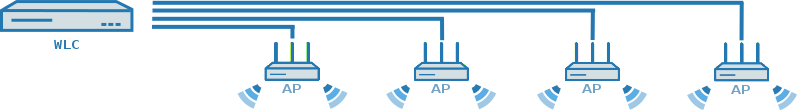
\includegraphics[width=0.8\columnwidth]{figures/wlc_aps}
	  \caption{Common \ac{AP} deployment where APs are connected to backbone via wire.}
	  \label{fig:wlc_aps}
	\end{figure}
	The procedure of establishing such a network can be described as follows:
	\begin{enumerate}
	 \item APs search for a \ac{WLC} on the wired network by \ac{IP}-broadcast.
	 \item After the authentication of the \ac{AP} the \ac{AP} establishes a secure (\ac{DTLS}) channel to the \ac{WLC} through a \ac{CAPWAP}-Layer.
	 \item \ac{AP} receives a configuration from the \ac{WLC} through the secure channel and reconfigures itself accordingly.
	\end{enumerate}
	
      \subsubsection{Automatic \ac{WDS}}
	\label{autowdsbasic}
	AutoWDS is an extension to the \ac{WLC}-aided configuration by also allowing such a configuration procedure over wireless links instead of solely wired connections.
            
	\begin{figure}[h!]
	  \centering
	  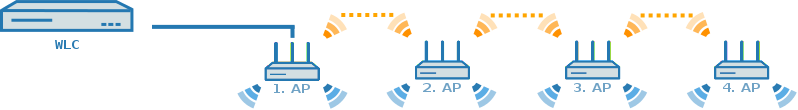
\includegraphics[width=0.8\columnwidth]{figures/autowds}
	  \caption{AutoWDS configuration setup. Only one AP is connected to the backbone via wire. 
	    Other APs use their radios to connect to APs that are connected to the backbone via wire (first \ac{AP}) or relay-APs (2nd \ac{AP}).}
	  \label{fig:autowds}
	\end{figure}
	
	The procedure is enhanced accordingly:
	
	\begin{enumerate}
	  \item The first \ac{AP} finds a \ac{WLC} and proceeds as before. Additionally it announces its connection to the \ac{WLC} over its radios to other APs.
	  
	  \item The second \ac{AP} does not find a \ac{WLC} on its \ac{LAN}-interface and extends its search on the radios. 
	    There it receives the announcement of the first \ac{AP}.
	    Consequently it connects itself to the first AP by client-infrastructure-mode and offers the same network on its other radios.
	    
	  \item The second \ac{AP} establishes a secure connection (\ac{WPA2}) to the first \ac{AP} and continues its search for a \ac{WLC} over this link, 
	    where it finds the \ac{WLC} and also receives a configuration (\ac{CAPWAP} / \ac{DTLS}) and proceeds as \ac{AP} one.
	    
	  \item Gradually all the APs connect each other to the backbone, receive a configuration and spread the \ac{WLAN} network.
	\end{enumerate}
	
\section{Graph-theoretic Basics}
  In the following we will recall the definitions of graphs, directed / weighted edges and paths in a graph.
  \begin{itemize}
    \item A graph in graph theory is a set of nodes and edges between these nodes.
    \item A directed graph / digraph has directions on its edges defined.
    \item A weighted graph has weights attached to its edges.
    \item A graph is called connected if every pair of nodes is connected. 
      Two nodes A,B are connected if there exists a path from A to B.
      A path is a sequence of edges where each edge has to fit to the next, like the game of domino.
  \end{itemize}

  \begin{figure}[th!]
    \centering
    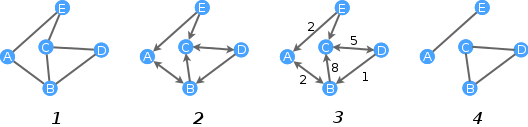
\includegraphics[width=0.8\columnwidth]{figures/graphen.png}
    \caption{Example graphs - 1: undirected 2: directed 3:weighted, directed 4: disconnected}
    \label{fig:graphen}
  \end{figure}

  We choose to use graph theory to represent our networks structures for two reasons:
  \begin{itemize}
   \item We are able to easily express all the relevant parts of a network directly in a graph without any modifications to graph theory,  
   like APs and modules by nodes, links between APs with edges and signal to noise ratios with weightedness of edges. 
    
   \item Graph theory is a well researched field and a lot of problems in it can be solved efficiently and intuitively 
    as we will see later with the \ac{DJP} algorithm.
  \end{itemize}
    
  \subsection{\emph{k}-Vertex-connectivity, \emph{k}-Edge-connectivity}
    A graph is called \textit{k-vertex-connected} if there exists a set of \textit{k} vertices whose removal disconnects parts of the graph.
    A graph is called \textit{k-edge-connected} if the graph is still connected after the removal of \textit{k} edges.
    \begin{figure}[th!]
      \centering
      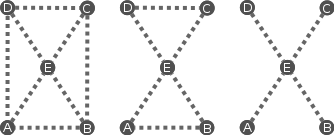
\includegraphics[width=0.5\columnwidth]{figures/connectivity.png}
      \caption{Graph-connectivity attributes from left to right: 2-vertex and 2-edge, 0-vertex and 1-edge, 0-vertex and 0-edge}
      \label{fig:connectivity}
    \end{figure}
    
\newpage
    
  \subsection{Minimum Spanning Tree}
    A spanning tree is a subgraph for a given graph which contains all nodes of the original graph, but only the necessary and edge-weight minimal 
    subset of edges which are needed to connect each node to the component. In order to find a minimum spanning tree for a non-negative weighted 
    graph we use the \ac{DJP} algorithm \cite{prim} \cite{jarnik}. It works as described by the following:
    
    \begin{enumerate}
     \item Initialize the minimum tree with a single, randomly chosen vertex from the given graph.
     
     \item For all edges originating the set of nodes in the minimum tree to nodes which have not been visited yet, 
      select the edge with the lowest score and add it and its nodes to the minimum tree.
      
     \item Repeat step two as long as not all vertices of the given graph are visited.
    \end{enumerate}
    
    \begin{figure}[th!]
      \centering
      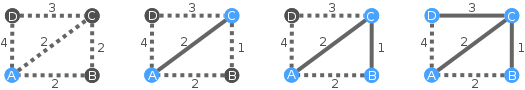
\includegraphics[width=0.8\columnwidth]{figures/djp.png}
      \caption{\ac{DJP} algorithm calculating a minimal spanning tree.}
      \label{fig:djp}
    \end{figure}
    
  \subsection{Significance of COLORING}
    Other pursuits of this problem including \cite{BFS-CA}, \cite{CTA}, \cite{caa_tricky} and \cite{katzela} mention a kinship to the problem COLORING on graphs.
    On the other hand, \cite{caa_tricky} also mentions:
    
    \begin{quote}
      At first glance, this problem appears to be a graph-coloring problem. However, standard graph-coloring algorithms cannot really capture the specification and constraints 
      of the channel assignment problem. A node-multi-coloring formulation fails to capture [...] communicating nodes need[ing] a common color. On the other hand,
      an edge-coloring formulation fails to capture the [...] constraint where no more than \textit{q} (number of NICs per node) colors can be incident to a node.
      While a constraint edge-coloring might be able to roughly model the remaining constraints, it is incapable of satisfying the constraint of limited channel capacity.
    \end{quote}
    
    In addition to the modeling problems a potential result of such a COLORING solution still would not make a point on the topology to use,
    as COLORING works on given network graphs and therefore topologies, but we also have to decide how to create and select the network topology.
    As a consequence, this formal problem or solutions to it are not considered in our work.
    
  \subsection{Mapping Network to Graph}
    For our purposes we will use the following mapping from devices and modules to a undirected, weighted graph.
    Each \ac{AP} and each module of our APs is represented by a node.
    
    For each \ac{AP} we add edges with a special attribute "artificial" 
    to each module of its corresponding \ac{AP} and describe those edges as artificial or device-module-edges.
    Those edges also have their \ac{SNR} value set to the maximum value possible. 
    
    If two modules are within receive range of each other, 
    we add an edge between the corresponding module nodes with the average signal-to-noise ratio as the edge-weight.
    We call those edges module-module connections or real connections.
    Since the average of the two \ac{SNR} values might not describe all scenarios well enough (in a scenario where \ac{SNR} values differ broadly),
    we easily can adjust the edge-weight to the minimum or maximum of both values.
    
    Furthermore we ignore one-sided discoveries, i.e. one module receives some beacons of the other module, but not the other way round.
        
    \begin{figure}[th!]
      \centering
      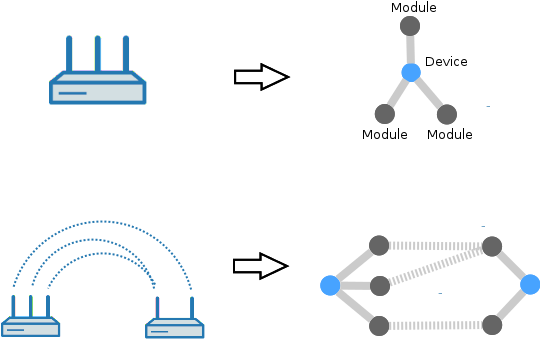
\includegraphics[width=0.7\columnwidth]{figures/apgraph.png}
      \caption{Graph representation of one (upper) and two connected APs (lower).}
      \label{fig:apgraph}
    \end{figure}
